\documentclass[10pt,aspectratio=169]{beamer}
\usetheme{metropolis}
\usepackage{booktabs}
\usepackage{siunitx}
\usepackage{graphicx}
\usepackage{xcolor}
\usepackage{tikz}
\usetikzlibrary{shapes.geometric, arrows.meta, positioning, fit, backgrounds}
\definecolor{good}{HTML}{2E7D32}
\definecolor{bad}{HTML}{C62828}
\definecolor{llmblue}{HTML}{1565C0}
\newcommand{\gd}[1]{\textcolor{good}{#1}}
\newcommand{\bd}[1]{\textcolor{bad}{#1}}
\metroset{block=fill}

\tikzset{
  llm/.style={rectangle, rounded corners, draw=llmblue, line width=0.8pt, fill=llmblue!8, align=center, font=\scriptsize, inner sep=4pt},
  frozen/.style={rectangle, rounded corners, draw=good, line width=0.9pt, fill=good!10, align=center, font=\scriptsize, inner sep=4pt},
  data/.style={rectangle, draw=gray!70, fill=gray!8, align=center, font=\scriptsize\ttfamily, inner sep=4pt},
  gate/.style={diamond, aspect=2, draw=bad, line width=0.9pt, fill=bad!8, align=center, font=\scriptsize, inner sep=1pt},
  arr/.style={-{Stealth[length=2mm]}, line width=0.7pt, gray!70},
}

\title{Centri --- Circular-Motion Video Pipeline}
\subtitle{Improvements Reports: Fri Jun 5 $\to$ Mon Jun 8, 2026}
\author{NCU HwangLab \\ Damar \& Claude Opus 4.8 Max}
\date{2026-06-08, 3:14 AM GMT+8 (Asia/Taipei)}

\begin{document}

\maketitle

\begin{frame}{Executive summary}
\begin{itemize}
  \item \textbf{Symptom:} the same turntable video produced a \emph{different} \texttt{stats.json} every run --- different schema, different numbers, sometimes invalid JSON.
  \item \textbf{Root cause:} the LLM was \emph{re-authoring the physics math} on every job.
  \item \textbf{Fix philosophy:} \emph{preseed frozen, vetted code} into each job (like the sidecar) --- keep the LLM only for perception.
\end{itemize}
\vspace{0.3em}
\begin{block}{Headline results}
\begin{itemize}
  \item \texttt{stats.json}: \bd{28 schemas / 17 invalid-NaN} $\to$ \gd{1 locked schema, 0 NaN}
  \item Same-video spread (IMG\_3071 period): \bd{26\%} $\to$ \gd{0\% (byte-identical)}
  \item Accuracy vs phone gyro: \gd{0.2--0.4\%} on all three videos
  \item Processing time: \bd{$\sim$30 min} $\to$ \gd{$\sim$8 min}; correctness now \emph{enforced}, not requested
\end{itemize}
\end{block}
\end{frame}

\begin{frame}{The system at a glance}
\begin{columns}[T]
\begin{column}{0.5\textwidth}
\textbf{Harness / models}
\begin{itemize}\scriptsize
  \item \texttt{pi} agentic CLI; the model writes \& runs Python per job
  \item LLM: \textbf{Qwen3.6-35B-A3B} (MoE) via llama.cpp @ \texttt{10.0.0.2:8083}, reasoning on
  \item Tracking: \textbf{SAM3} (Grounding DINO + DETR) @ \texttt{10.0.0.1:8086}, \textbf{1 cached call/job}
  \item FastAPI + Celery (concurrency 1) + Redis; Flutter app (Nokia)
\end{itemize}
\end{column}
\begin{column}{0.5\textwidth}
\textbf{Agents}
\begin{itemize}\scriptsize
  \item Orchestrator (Steps 1--6)
  \item Subagent A --- video annotation
  \item Subagent B --- figure generation
  \item Subagent C --- question bank
  \item Subagent D --- figure visual QA \emph{(new, retry-only)}
  \item Extractor --- output manifest
  \item \gd{\textbf{Frozen \texttt{analysis/} --- no LLM, owns all kinematics}}
\end{itemize}
\end{column}
\end{columns}
\end{frame}

\section{Architecture}

\begin{frame}{Pipeline flow --- where the LLM stops and frozen code starts}
\centering
\resizebox{\textwidth}{!}{%
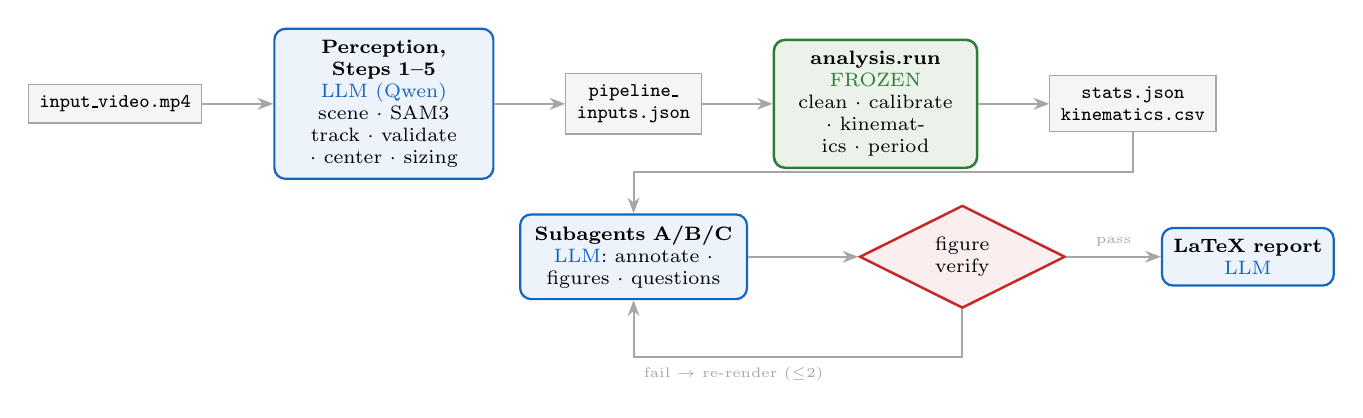
\begin{tikzpicture}[node distance=6mm and 9mm]
\node[data] (vid) {input\_video.mp4};
\node[llm, right=of vid, text width=2.5cm] (perc) {\textbf{Perception, Steps 1--5}\\\textcolor{llmblue}{LLM (Qwen)}\\scene $\cdot$ SAM3 track $\cdot$ validate $\cdot$ center $\cdot$ sizing};
\node[data, right=of perc] (contract) {pipeline\_\\inputs.json};
\node[frozen, right=of contract, text width=2.3cm] (run) {\textbf{analysis.run}\\\gd{FROZEN}\\clean $\cdot$ calibrate $\cdot$ kinematics $\cdot$ period};
\node[data, right=of run] (stats) {stats.json\\kinematics.csv};
\draw[arr] (vid)--(perc); \draw[arr] (perc)--(contract); \draw[arr] (contract)--(run); \draw[arr] (run)--(stats);

\node[llm, below=10mm of contract, text width=2.6cm] (subs) {\textbf{Subagents A/B/C}\\\textcolor{llmblue}{LLM}: annotate $\cdot$ figures $\cdot$ questions};
\node[gate, right=14mm of subs, text width=1.4cm] (gate) {figure\\verify};
\node[llm, right=12mm of gate, text width=1.9cm] (rep) {\textbf{LaTeX report}\\\textcolor{llmblue}{LLM}};
\draw[arr] (stats.south) -- ++(0,-5mm) -| (subs.north);
\draw[arr] (subs)--(gate);
\draw[arr] (gate)-- node[above,font=\tiny]{pass} (rep);
\draw[arr] (gate.south) -- ++(0,-6mm) -| node[below right,font=\tiny]{fail $\to$ re-render ($\le$2)} (subs.south);
\end{tikzpicture}}
\par\vspace{0.4em}
\footnotesize \textcolor{llmblue}{Blue = LLM / non-deterministic} \quad\quad \gd{Green = frozen / deterministic} \quad\quad \texttt{grey = data artifact}
\end{frame}

\begin{frame}{The seam + three determinism guarantees}
\centering
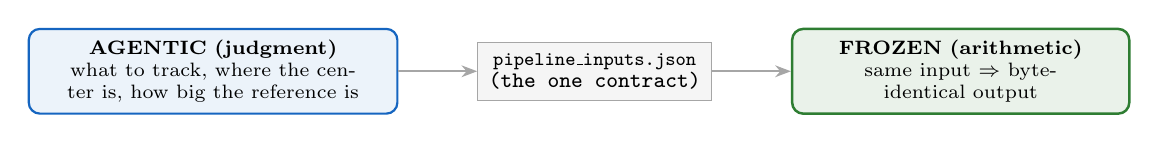
\begin{tikzpicture}[node distance=5mm]
\node[llm, text width=4.4cm] (a) {\textbf{AGENTIC (judgment)}\\ what to track, where the center is, how big the reference is};
\node[data, right=10mm of a] (c) {pipeline\_inputs.json\\\footnotesize(the one contract)};
\node[frozen, right=10mm of c, text width=4.0cm] (f) {\textbf{FROZEN (arithmetic)}\\ same input $\Rightarrow$ byte-identical output};
\draw[arr] (a)--(c); \draw[arr] (c)--(f);
\end{tikzpicture}
\vspace{0.6em}
\begin{block}{Baked into the frozen layer}
\textbf{1. Seeded RANSAC RNG} --- identical circle fit every run.\\
\textbf{2. Single $\omega$ source} --- one series drives active-detection, summary, period \emph{and} phases (the old code used two).\\
\textbf{3. Locked schema + \texttt{allow\_nan=False}} --- same keys every run; a stray NaN \emph{raises} instead of shipping invalid JSON.
\end{block}
\end{frame}

\section{The frozen ``preseeded'' code, in detail}

\begin{frame}{How it is seeded into every job}
\centering
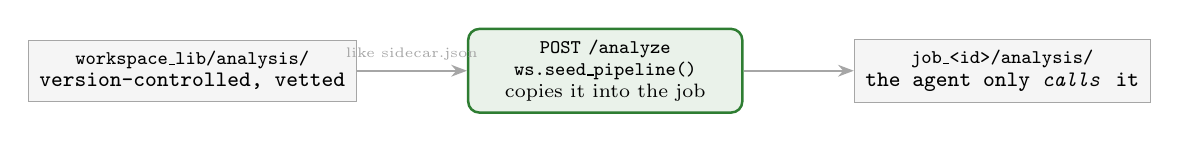
\begin{tikzpicture}[node distance=8mm]
\node[data] (lib) {\textbf{workspace\_lib/analysis/}\\\footnotesize version-controlled, vetted};
\node[frozen, right=14mm of lib, text width=3.2cm] (seed) {\texttt{POST /analyze}\\\texttt{ws.seed\_pipeline()}\\copies it into the job};
\node[data, right=14mm of seed] (job) {job\_<id>/analysis/\\\footnotesize the agent only \emph{calls} it};
\draw[arr] (lib)--node[above,font=\tiny]{like sidecar.json}(seed); \draw[arr] (seed)--(job);
\end{tikzpicture}
\par\vspace{0.5em}
\footnotesize The agent is \emph{forbidden} to edit or reimplement \texttt{analysis/} (HARD RULE in the orchestrator). Its job ends at writing \texttt{pipeline\_inputs.json}; Step 6 is just \texttt{python -m analysis.run}.
\end{frame}

\begin{frame}{The modules (what each one owns)}
\centering\scriptsize
\begin{tabular}{@{}p{2.6cm}p{9.3cm}@{}}
\toprule
module & responsibility \\
\midrule
\texttt{common.py} & seeded RNG (\texttt{RANDOM\_SEED=20240517}), logging, validation flags, step/progress markers \\
\texttt{contract.py} & load + validate \texttt{pipeline\_inputs.json} $\to$ \texttt{Inputs}; \gd{owns the display$\to$cropped transform} (\texttt{coordinate\_space}+\texttt{roi\_crop}) for trajectory \emph{and} center together \\
\texttt{geometry.py} & RANSAC circle fit (seeded) + \gd{degeneracy guard}; calibration \texttt{px\_per\_m}; center selection; outlier rejection from the trusted center \\
\texttt{kinematics.py} & \gd{single $\omega$ source} (unwrap $\to$ Savitzky-Golay $\to$ gradient $\to$ median); active detection; period \& FFT; phase segmentation; \gd{polar short-gap fill} \\
\texttt{writer.py} & locked \texttt{stats.json} (\texttt{allow\_nan=False}) + \texttt{kinematics.csv} (now incl. cropped \texttt{x\_px,y\_px}); post-hoc sanity gate \\
\texttt{verify\_figures.py} & \gd{deterministic figure-QA gate} (new) --- plotted bounds vs \texttt{kinematics.csv} \\
\texttt{run.py} & \texttt{python -m analysis.run} entry point; emits progress \\
\texttt{render/} & vetted annotation reference for the video subagent \\
\bottomrule
\end{tabular}
\end{frame}

\begin{frame}{Data flow inside \texttt{analysis.run}}
\centering
\resizebox{\textwidth}{!}{%
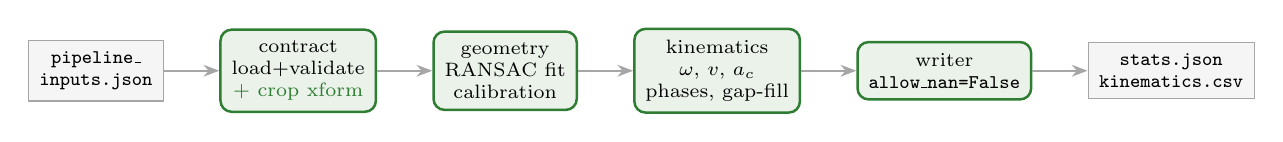
\begin{tikzpicture}[node distance=5mm and 7mm]
\node[data] (in) {pipeline\_\\inputs.json};
\node[frozen, right=of in] (con) {contract\\load+validate\\\gd{+ crop xform}};
\node[frozen, right=of con] (geo) {geometry\\RANSAC fit\\calibration};
\node[frozen, right=of geo] (kin) {kinematics\\$\omega$, $v$, $a_c$\\phases, gap-fill};
\node[frozen, right=of kin] (wr) {writer\\\texttt{allow\_nan=False}};
\node[data, right=of wr] (out) {stats.json\\kinematics.csv};
\draw[arr](in)--(con);\draw[arr](con)--(geo);\draw[arr](geo)--(kin);\draw[arr](kin)--(wr);\draw[arr](wr)--(out);
\end{tikzpicture}}
\par\vspace{0.5em}
\footnotesize Every value in \texttt{stats.json} is traceable to this chain; no LLM touches any of it. Result: \gd{same \texttt{pipeline\_inputs.json} $\Rightarrow$ byte-identical \texttt{stats.json}}.
\end{frame}

\section{The problem \& determinism overhaul}

\begin{frame}{Before: agent-authored math (30 historical jobs)}
\begin{block}{Schema integrity}
\bd{28 distinct \texttt{stats.json} schemas} across 30 jobs; \bd{17 contained bare \texttt{NaN}} (invalid JSON).
\end{block}
\centering\small
\begin{tabular}{lccccc}
\toprule
Video & runs & \texttt{period\_s} spread & \texttt{mean\_omega} & \texttt{stable\_omega} & \texttt{drift\_px} \\
\midrule
IMG\_3071 & 15 & \bd{0.793--1.002 (26\%)} & 6.16--8.25 & 0.60--11.1 & 0--116 \\
IMG\_3072 & 5  & 1.486--1.487 (0\%) & 4.681 & 0.82--4.99 & 13--393 \\
IMG\_3075 & 5  & 1.102 (0\%) & 5.827 & 2.89--6.07 & \bd{8.9--1013} \\
\bottomrule
\end{tabular}
\par\vspace{0.5em}
\footnotesize \texttt{stable\_omega} and \texttt{center\_drift} swung wildly on \emph{every} video; schemas never repeated; IMG\_3071's core period swung 26\%.
\end{frame}

\begin{frame}{Root cause \& the decision}
\begin{block}{Root cause}
The orchestrator told the agent to \emph{compute} kinematics and \emph{write} \texttt{stats.json}, but left the math as prose pseudo-code / a stub. So the LLM \textbf{re-derived the analysis every run}, differently each time. (Unseeded RANSAC $\to$ the 8.9$\to$1013 drift; two $\omega$ computations $\to$ \texttt{stable\_omega} instability.)
\end{block}
\begin{block}{The decision (user's framing)}
\emph{``Preseed the workspace with quality code, just like sidecar behaviour.''} Demote the arithmetic to a fixed library the agent \emph{calls}; keep the LLM where it adds judgment.
\end{block}
\end{frame}

\begin{frame}{Result: determinism + accuracy (3$\times$ per video)}
All 9 jobs: \gd{\texttt{schema\_version: 1}, zero \texttt{NaN}}.
\centering\small
\begin{tabular}{lccccc}
\toprule
Video & \texttt{period\_s} & \texttt{mean\_omega} & vs gyro & drift & determinism \\
\midrule
IMG\_3071 & \gd{0.839 (0\%)} & \gd{7.372 (0\%)} & \gd{0.2\%} & 0.0 & \gd{identical $\times$3} \\
IMG\_3072 & \gd{1.438 (0\%)} & \gd{4.827 (0\%)} & \gd{0.4\%} & 28.4 & \gd{identical $\times$3} \\
IMG\_3075 & 1.102--1.150 (4.3\%) & 5.79--5.89 (1.7\%) & \gd{0.3\%} & 13/171 & r1$\equiv$r3 \\
\bottomrule
\end{tabular}
\par\vspace{0.5em}
\begin{columns}[T]\begin{column}{0.5\textwidth}\centering\footnotesize
\begin{tabular}{lcc}
schemas/30 & \bd{28} & \gd{1} \\
NaN JSON & \bd{17} & \gd{0} \\
3071 spread & \bd{26\%} & \gd{0\%} \\
drift range & \bd{8.9$\to$1013} & \gd{0.0} \\
\end{tabular}
\end{column}\begin{column}{0.5\textwidth}\footnotesize
IMG\_3075 run2's wobble is \emph{SAM tracking} variance (a different trajectory that run), \emph{not} the math --- exactly the separation the redesign created.
\end{column}\end{columns}
\end{frame}

\section{Bugs caught \& fixed}

\begin{frame}{RANSAC degeneracy --- caught by the spot-check}
The new \emph{plumbing} worked first try; \bd{but job 1's numbers were garbage:}
\centering\small
\begin{tabular}{lccc}
\toprule
metric & \bd{buggy} & \gd{fixed} & gyro \\
\midrule
\texttt{center\_drift\_px} & 8045 & \gd{0.0} & --- \\
\texttt{r\_fit\_m} & 3.13 m & \gd{0.148} & --- \\
outliers rejected & 163/321 & \gd{0} & --- \\
\texttt{mean\_omega} & 0.0 & \gd{7.372} & 7.357 \\
\texttt{period\_s} & 0.0 & \gd{0.839} & 0.854 \\
\bottomrule
\end{tabular}
\par\vspace{0.5em}
\footnotesize
\textbf{Cause:} seeded RANSAC locked onto a \emph{degenerate giant circle} (huge radius $\approx$ locally straight $\to$ ``fits'' arc points), poisoning the outlier step. \emph{Determinism made it reproducible, not correct.}\\
\textbf{Fix:} derive radius \& outliers from the \emph{median distance to the trusted center}; reject implausible fits (\texttt{ransac\_fit\_rejected}).
\end{frame}

\begin{frame}{Coordinate-space determinism bug (IMG\_3072)}
\begin{columns}[T]
\begin{column}{0.46\textwidth}
\centering\small
\begin{tabular}{lcc}
\toprule
 & v1 & \gd{v2 fixed} \\
\midrule
\texttt{mean\_omega} & 0.7\% & \gd{0.0\%} \\
\texttt{period\_s} & \bd{14.6\%} & \gd{0.0\%} \\
\texttt{stable\_omega} & \bd{81\%} & \gd{0.0\%} \\
\bottomrule
\end{tabular}
\par\vspace{0.4em}
\footnotesize Raw SAM tracking was \emph{byte-identical} across the two runs --- so this was \emph{not} perception.
\end{column}
\begin{column}{0.54\textwidth}
\footnotesize
\textbf{Cause:} the agent applied the display$\to$cropped transform \emph{by hand, inconsistently} --- one run subtracted the \SI{87}{px} crop offset (\texttt{y\_off}) from the trajectory, one didn't, while the center stayed cropped.\\[0.3em]
\textbf{Fix:} move the \emph{last} coordinate transform off the LLM. The contract carries trajectory \emph{and} center in full-frame space; \texttt{contract.py} subtracts the offset for \emph{both together}. That class of bug is now structurally impossible.
\end{column}
\end{columns}
\end{frame}

\section{Figures \& verification}

\begin{frame}{The figure bug --- circle floated off the points}
\footnotesize The figures subagent plotted the trajectory from \texttt{api\_cache.json} (full-frame) while drawing the center from cropped \texttt{stats.json}. A prompt HARD RULE \emph{did not hold} (twice).
\begin{columns}[T]
\begin{column}{0.5\textwidth}\centering
\bd{Before}\\\includegraphics[height=0.62\textheight]{/tmp/v2_trajectory.png}
\end{column}
\begin{column}{0.5\textwidth}\centering
\gd{After}\\\includegraphics[height=0.62\textheight]{/tmp/v3_trajectory.png}
\end{column}
\end{columns}
\end{frame}

\begin{frame}{Verification flow (a + c) --- correctness enforced}
\centering
\resizebox{0.78\textwidth}{!}{%
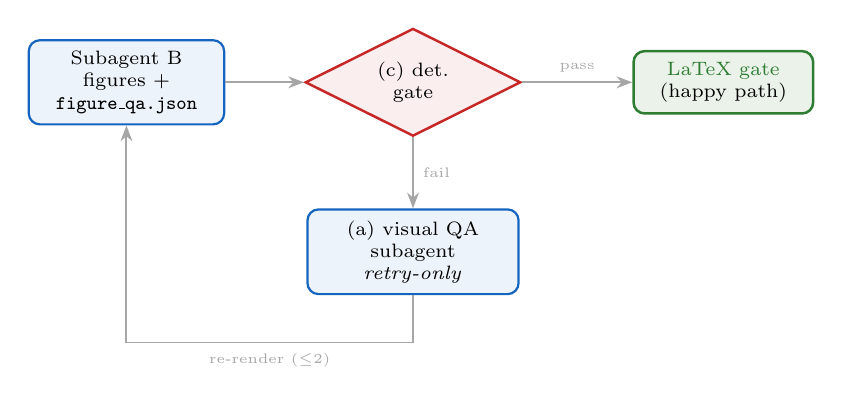
\begin{tikzpicture}[node distance=6mm and 10mm]
\node[llm, text width=2.2cm] (b) {Subagent B\\figures + \texttt{figure\_qa.json}};
\node[gate, right=of b, text width=1.5cm] (det) {(c) det.\\gate};
\node[frozen, right=14mm of det, text width=2.0cm] (ok) {\gd{LaTeX gate}\\(happy path)};
\node[llm, below=9mm of det, text width=2.4cm] (vqa) {(a) visual QA\\subagent\\\emph{retry-only}};
\draw[arr](b)--(det);
\draw[arr](det)--node[above,font=\tiny]{pass}(ok);
\draw[arr](det.south)--node[right,font=\tiny]{fail}(vqa);
\draw[arr](vqa.south) -- ++(0,-6mm) -| node[below,font=\tiny,pos=0.25]{re-render ($\le$2)} (b.south);
\end{tikzpicture}}
\par\vspace{0.2em}
\begin{block}{Two checks}
\footnotesize
\textbf{(c) Deterministic gate} (\texttt{verify\_figures.py}, every job, instant): the subagent emits \texttt{figure\_qa.json} with the bounds it plotted; the gate recomputes truth from \texttt{kinematics.csv} and \bd{fails} on a \texttt{y\_off} offset. \emph{Tested: PASS on cropped, FAIL on +\SI{161}{px}.}\\
\textbf{(a) Visual QA subagent} (multimodal, only on a gate failure): ``is the circle on the points? labels OK?'' $\to$ feedback into the retry.
\end{block}
\end{frame}

\section{Robustness \& physics quality}

\begin{frame}{Short-gap fill for motion-blur dropouts}
Fast spins blur the object $\to$ SAM3 drops frames $\to$ \texttt{NaN} gaps in $\omega(t)$.
\begin{center}
\includegraphics[width=0.92\textwidth]{/tmp/omega_beforeafter.png}
\end{center}
\vspace{-0.3em}
\footnotesize
\textbf{Bounded polar interpolation:} bridge interior gaps $\le$\SI{0.2}{s} (12 frames) in $(\theta,r)$ about the center (points land \emph{on} the orbit); only between two real detections; flagged \texttt{interpolated\_short\_gaps}. \gd{Deterministic} (no RNG); coverage reflects real detections only; long gaps stay honest. IMG\_3072 period 1.44$\to$\gd{1.37 s} (gyro 1.307).
\end{frame}

\begin{frame}{Runaway guard + log compression (today)}
A live job hit an LLM \textbf{generation loop} in the LaTeX step:
\centering\small
\begin{tabular}{lr}
\toprule
artifact & value \\
\midrule
\texttt{pi\_events.jsonl} size & \bd{$\approx$11.4 GB} \\
event lines & \bd{76{,}797} \\
repeated event & \emph{``Let me create the LaTeX file\ldots''} \\
job state & stuck 72\% $\sim$25 min (would hang to 90-min timeout) \\
\midrule
\gd{after guard} & \gd{killed at 1 GB ($\sim$1--2 min); log gzip'd $\sim$50--100$\times$} \\
\bottomrule
\end{tabular}
\par\vspace{0.5em}
\footnotesize Figures, the \texttt{figure\_verify} gate, questions and the annotated video had \emph{all completed correctly} first --- the failure was isolated to the (still LLM-authored) LaTeX step, now bounded.
\end{frame}

\section{App \& auto-detect}

\begin{frame}{Auto-suggest / detect --- the failures, then the fix}
\begin{block}{What was wrong}
\begin{itemize}\footnotesize
  \item \bd{Loose boxes:} \texttt{/suggest-scene} used the \textbf{VLM only} --- approximate boxes that didn't hug the object. SAM3 (the precise detector) was a \emph{separate} ``Check the app can see them'' tap.
  \item \bd{Hard failure (502):} \texttt{/suggest-scene} dialed a \emph{dead} inference host (\texttt{PI\_INFERENCE\_URL} 192.168.1.205); auto-detect just errored on the phone.
\end{itemize}
\end{block}
\begin{block}{The fix --- chain VLM $\to$ SAM3 server-side}
\begin{itemize}\footnotesize
  \item VLM does \emph{semantics} (names the object, picks the platform, finds the center); SAM3 then \emph{grounds those labels} and returns \gd{tight boxes} --- in one call.
  \item Best-effort (falls back to the VLM box on a SAM miss); rotation-center stays the VLM pivot (a centroid is a different point).
  \item Fixed the inference URL $\to$ \gd{10.0.0.2:8083}. \gd{Verified: suggest boxes match pure-SAM3 to $\sim$1\%.}
\end{itemize}
\end{block}
\end{frame}

\begin{frame}{Other app improvements}
\begin{itemize}
  \item \textbf{De-jargoned for students/teachers:} ``SAM3'' $\to$ ``the app can see them''; the ``known-size object / ruler'' rule reframed to \emph{the spinning platform itself} (5 UI strings + VLM prompt + overlay tag).
  \item \textbf{Upload progress bar:} live \% modal while the video uploads.
  \item \textbf{History view:} friendly title (not the raw UUID), \texttt{2m 54s} time format, inline progress bar, plus \texttt{object\_name} + ``2 min ago'' (new backend fields).
  \item \textbf{Removed dead \texttt{bbox\_center\_px}} sidecar field (backend never used it).
  \item \textbf{Capture tips:} bright light, moderate spin --- reduce blur dropouts at the source.
\end{itemize}
\end{frame}

\section{Bicycle template --- translation check}

\begin{frame}{Bicycle still good: a different geometry tracks \& measures}
\begin{columns}[T]
\begin{column}{0.58\textwidth}\centering
\includegraphics[width=0.49\linewidth]{/home/damar/centri/screenshot/bike-1.png}\hfill
\includegraphics[width=0.49\linewidth]{/home/damar/centri/screenshot/bike-2.png}
\par\footnotesize Annotated frames: tracked red marker, fitted circle, radius vector.
\end{column}
\begin{column}{0.42\textwidth}\footnotesize
\begin{tabular}{ll}
\toprule
rotation & \gd{CW (correctly signed)} \\
\texttt{mean\_omega} & $-5.12$ rad/s \\
\texttt{period\_s} & 1.18 s \\
coverage & 93.8\% (11 gap-filled) \\
\bottomrule
\end{tabular}
\par\vspace{0.4em}
The frozen pipeline handles the bicycle wheel: \gd{CW direction signed correctly}, $\omega$/period resolved, short-gap fill active.\\[0.3em]
\footnotesize No sidecar size $\to$ tyre size \emph{estimated} (\texttt{world\_knowledge}), so $v$/$a_c$ are scale-shifted; $\omega$/period are scale-free and correct.
\end{column}
\end{columns}
\end{frame}

\section{Validation \& scope}

\begin{frame}{Ground truth, accuracy \& a clean regression}
\begin{columns}[T]
\begin{column}{0.5\textwidth}
\textbf{Phone gyro} (dev ground truth, never seen by the agent)
\centering\footnotesize
\begin{tabular}{lcc}
\toprule
Video & gyro $\omega$ & gyro $T$ \\
\midrule
IMG\_3071 & 7.357 & 0.854 \\
IMG\_3072 & 4.806 & 1.307 \\
IMG\_3075 & 5.811 & 1.081 \\
\bottomrule
\end{tabular}
\end{column}
\begin{column}{0.5\textwidth}
\textbf{Regression re-run (today)}
\begin{itemize}\footnotesize
  \item Turntable: \texttt{7.3722 / 0.8387} --- \gd{$\Delta$=0.0000, byte-identical} to known-good.
  \item Phone: 445 s ($\sim$7.4 min), figure gate passed, \emph{visual QA not needed} (happy path fast).
\end{itemize}
\end{column}
\end{columns}
\vspace{0.4em}
\begin{itemize}\footnotesize
  \item \texttt{mean\_omega} within \gd{0.2--0.4\%} of gyro on all three (old pipeline was $\sim$2.6\% off on IMG\_3072).
  \item $\omega$/period are calibration-independent $\to$ they validate the tracking-only pipeline; the product never uses sensor data.
\end{itemize}
\end{frame}

\begin{frame}{Honest scope --- what is \emph{not} solved}
\begin{itemize}
  \item \textbf{Perception (SAM3) is still non-deterministic.} The frozen math is byte-identical \emph{for identical tracking}; residual spread points at tracking, not math.
  \item \texttt{stable\_mean\_omega} is the most fragile metric (phase-regression sensitive to noise). Prefer \texttt{mean\_omega} / \texttt{period} for the pilot.
  \item \textbf{Reference physical size} matters for linear values ($v$, $a_c$); $\omega$/period are scale-free.
  \item \textbf{The LaTeX report is still LLM-authored} --- loop risk now \emph{guarded}; a frozen template would remove it entirely (candidate next step).
\end{itemize}
\end{frame}

\begin{frame}{Bottom line}
\begin{block}{Determinism \& accuracy}
Same video $\to$ same data: \gd{1 locked schema, 0 NaN}, byte-identical on clean tracking; \gd{0.2--0.4\%} agreement with the phone gyro.
\end{block}
\begin{block}{Speed \& safety}
\gd{$\sim$30 min $\to$ $\sim$8 min} per job; runaway loops now bounded ($\le$1 GB), event logs compressed.
\end{block}
\begin{block}{Architecture}
Every position-space conversion lives inside the \gd{frozen seam} --- none on the LLM. Correctness is \emph{enforced} by deterministic gates, not requested by prompt.
\end{block}
\end{frame}

\section{App screenshots}

\begin{frame}{App screenshots 1/3 --- capture and frame selection}
\begin{columns}[T]
\begin{column}{0.33\textwidth}\centering
\includegraphics[width=\linewidth]{/home/damar/centri/screenshot/1.png}\\
\scriptsize Capture / upload
\end{column}
\begin{column}{0.33\textwidth}\centering
\includegraphics[width=\linewidth]{/home/damar/centri/screenshot/2.png}\\
\scriptsize Object marking
\end{column}
\begin{column}{0.33\textwidth}\centering
\includegraphics[width=\linewidth]{/home/damar/centri/screenshot/3.png}\\
\scriptsize Rotation centre
\end{column}
\end{columns}
\end{frame}

\begin{frame}{App screenshots 2/3 --- tracking and results}
\begin{columns}[T]
\begin{column}{0.33\textwidth}\centering
\includegraphics[width=\linewidth]{/home/damar/centri/screenshot/4.png}\\
\scriptsize Tracking in progress
\end{column}
\begin{column}{0.33\textwidth}\centering
\includegraphics[width=\linewidth]{/home/damar/centri/screenshot/5.png}\\
\scriptsize Results / worksheet
\end{column}
\begin{column}{0.33\textwidth}\centering
\includegraphics[width=\linewidth]{/home/damar/centri/screenshot/6.png}\\
\scriptsize Annotated video
\end{column}
\end{columns}
\end{frame}

\begin{frame}{App screenshots 3/3 --- history and tutor}
\begin{columns}[T]
\begin{column}{0.33\textwidth}\centering
\includegraphics[width=\linewidth]{/home/damar/centri/screenshot/8.png}\\
\scriptsize History view
\end{column}
\begin{column}{0.33\textwidth}\centering
\includegraphics[width=\linewidth]{/home/damar/centri/screenshot/9.png}\\
\scriptsize Progress feed
\end{column}
\begin{column}{0.33\textwidth}\centering
\includegraphics[width=\linewidth]{/home/damar/centri/screenshot/10.png}\\
\scriptsize Tutor / hints
\end{column}
\end{columns}
\end{frame}

\begin{frame}{Velocity--time plots 1/2}
\begin{columns}[T]
\begin{column}{0.48\textwidth}\centering
\includegraphics[width=\linewidth]{/home/damar/centri/agent-backend/workspaces/job_0fc2c525-cb00-4c66-a66d-2f2c5a36af1d/analysis_output/plots/v_t.png}\\
\scriptsize \texttt{job\_0fc2c5}
\end{column}
\begin{column}{0.48\textwidth}\centering
\includegraphics[width=\linewidth]{/home/damar/centri/agent-backend/workspaces/job_819db900-010c-46d3-9809-fd5e3a935e8a/analysis_output/plots/v_t.png}\\
\scriptsize \texttt{job\_819db9}
\end{column}
\end{columns}
\end{frame}

\begin{frame}{Velocity--time plots 2/2}
\begin{columns}[T]
\begin{column}{0.48\textwidth}\centering
\includegraphics[width=\linewidth]{/home/damar/centri/agent-backend/workspaces/job_ad73401c-89f3-443a-98eb-0e606ba8e6ac/analysis_output/plots/v_t.png}\\
\scriptsize \texttt{job\_ad7340}
\end{column}
\begin{column}{0.48\textwidth}\centering
\includegraphics[width=\linewidth]{/home/damar/centri/agent-backend/workspaces/job_250b2ebc-5bc8-4672-8d99-b8398eda2a5c/analysis_output/plots/v_t.png}\\
\scriptsize \texttt{job\_250b2e}
\end{column}
\end{columns}
\end{frame}

\begin{frame}{Trajectory plots 1/2}
\begin{columns}[T]
\begin{column}{0.48\textwidth}\centering
\includegraphics[width=\linewidth]{/home/damar/centri/agent-backend/workspaces/job_0fc2c525-cb00-4c66-a66d-2f2c5a36af1d/analysis_output/plots/trajectory.png}\\
\scriptsize \texttt{job\_0fc2c5}
\end{column}
\begin{column}{0.48\textwidth}\centering
\includegraphics[width=\linewidth]{/home/damar/centri/agent-backend/workspaces/job_819db900-010c-46d3-9809-fd5e3a935e8a/analysis_output/plots/trajectory.png}\\
\scriptsize \texttt{job\_819db9}
\end{column}
\end{columns}
\end{frame}

\begin{frame}{Trajectory plots 2/2}
\begin{columns}[T]
\begin{column}{0.48\textwidth}\centering
\includegraphics[width=\linewidth]{/home/damar/centri/agent-backend/workspaces/job_ad73401c-89f3-443a-98eb-0e606ba8e6ac/analysis_output/plots/trajectory.png}\\
\scriptsize \texttt{job\_ad7340}
\end{column}
\begin{column}{0.48\textwidth}\centering
\includegraphics[width=\linewidth]{/home/damar/centri/agent-backend/workspaces/job_250b2ebc-5bc8-4672-8d99-b8398eda2a5c/analysis_output/plots/trajectory.png}\\
\scriptsize \texttt{job\_250b2e}
\end{column}
\end{columns}
\end{frame}

\end{document}
